\section{Force, energy, work, momentum}

\subsection{Potential energy, conservative force, and work}

The \defn{work} done when a particle moves from $x_0$ to $x_1$ is defined to be
\begin{align*}
  W(x_0 \to x_1) := \int_{x_0}^{x_1} F(x) \dx.
\end{align*}

If this is independent of the path taken between $x_0$ and $x_1$, then we say the force is
\defn{conservative} and define the \defn{potential energy} at $x$, relative to $x_0$ to be
\begin{align*}
  V(x) &:= -\int_{x_0}^x F(x') \dx'.
\end{align*}
If the integral depends on the path taken, the potential energy is undefined.

\blue{A force moves something in space (causes an acceleration). Equivalently, something moves in
  space because a small displacement in some direction is associated with a lower potential
  energy. In fact, the force at a location \emph{is} the gradient in potential energy at that
  location.}

\begin{align*}
  F(x) &= -\frac{\d V(x)}{\dx} \\
  V(x) &= -\int_{x_0}^x F(x') \dx'
\end{align*}

\todo{Understand this}:

A force that depends only on position in one dimension is always conservative, because the integral
depends only on the endpoints. But a force that depends on e.g. time or velocity is
non-conservative. Friction is such a force because although it looks like a constant force
($\mu mg$), its direction (sign) is the opposite of the direction of velocity, so it is in fact
velocity-dependent.

Also, how is this so:
\begin{quote}
  \emph{Since friction always opposes the motion, the contributions to the $W = \int F \dx$ integral are
    always negative, so there is never any cancellation. The result is therefore a large negative
    number.}
\end{quote}

\subsection{Slowing down a moving object}

Facts:

\begin{enumerate}
\item The rate of change of momentum is determined by the net force acting on an object.
\item To slow something down, a force must be applied for some period of time.
\item To slow something which has momentum $p$, a strong force could be applied briefly, or a weaker
  force for a longer time.
\item ``Slow something down'' in those sentences could be replaced with ``change the velocity''. The
  change in velocity could be a change in direction, without a change in speed.
\end{enumerate}


Consider two bodies traveling in one dimension with masses and velocities $m_1, v_1$ and $m_2,
v_2$. Their momenta are identical: $m_1v_1 = m_2v_2$.

Suppose that mass $m_1 > m_2$, and therefore $v_1 < v_2$.

A force $F$ acts to slow them down. Over what length of time must the force be in effect?

The force causes accelerations (decelerations) $a_1 = F/m_1$ and $a_2 = F/m_2$. So we have velocity
functions
\begin{align*}
  \dv{x_1}{t} (t) &= v_1 - \frac{F}{m_1}t \\
  \dv{x_2}{t} (t) &= v_2 - \frac{F}{m_1}t,
\end{align*}
and we see that the velocities become equal to zero at the same time, i.e. when
$t = \frac{m_1v_1}{F} = \frac{m_2v_2}{F}$.

So, \blue{the length of time for which a force must be applied depends only on the momentum}; not on the
mass or velocity separately.

Now, how far does a mass travel while it is slowing down (i.e. over time $mv/F$)? This is
\begin{align*}
  x &= \int_{t=0}^{t=mv/F} \(v - \frac{F}{m}t\) \dt \\
    &= vt - \frac{F}{2m}t^2\Big|_{t=0}^{t=mv/F} \\
    &= \frac{mv^2}{F} - \frac{F}{2m}\frac{m^2v^2}{F^2} \\
    &= \frac{1}{2}mv^2/F.
\end{align*}

So, in order for a constant force $F$ to halt a mass $m$ with velocity $v$, the product of force and
the distance over which the force is applied (i.e. the work done) must equal the kinetic energy of
the mass $\frac{1}{2}mv^2$.

I.e. \blue{the distance over which the force must be applied depends on the kinetic energy}
$\frac{1}{2}mv^2$.

The lighter mass covers more distance while it is slowing down, because it has higher kinetic energy.

The following connections between force and momentum, and force and work/energy, make sense under
the FTC:
\begin{enumerate}
\item Force is the time derivative of momentum. The integral of force over time corresponds to change in momentum.
\item Force is the spatial derivative of potential energy. The integral of force over space
  (i.e. work) corresponds to change in potential energy.
\end{enumerate}



\subsection{Example: gravitational potential energy}

Consider two point masses $M$ and $m$, separated by a distance $r$. Newton's law of gravitation
states that there is a force between them of magnitude $-GMm/r^2$ (the force is attractive, hence
the negative sign).

The potential energy of the system at separation $r$, relative to separation $r_0$, is

\begin{align*}
  V(r) &= -\int_{r_0}^r F(r) \dr \\
       &= -\int_{r_0}^r \frac{-GMm}{r^2} \dr \\
       &= -\(\frac{GMm}{r} - \frac{GMm}{r_0}\).
\end{align*}

Typically in this situation we would choose $r_0 = \infty$ as the reference separation, so that
\begin{align*}
  V(r) = -\frac{GMm}{r}.
\end{align*}

\blue{Potential energy, relative to $r = \infty$, decreases as the two masses get closer: so the
  masses will approach each other. It's always negative because we have measured it relative to
  $r = \infty$, and any separation is more favorable than infinitely large separation.}

\begin{question*}
  What is the gravitational potential energy of a mass $m$ at a height $y$, relative to the Earth's
  surface?
\end{question*}

\begin{proof}
  Let the mass and radius of Earth be $M$ and $R$. Then
  \begin{align*}
    V(y) &= -\(\frac{GMm}{R + y} - \frac{GMm}{R}\) \\
         &= GMm(\frac{R + y - R}{R^2 + Ry}) \\
   &\approx \frac{GMmy}{R^2},
  \end{align*}
  for $y << R$. Recall that the gravitational acceleration of a particle of mass $m$ is $g = \frac{GM}{R^2}$. So
  we can write this in terms of $g$ as
  \begin{align*}
  V(y) &\approx mgy.
  \end{align*}
\end{proof}
\blue{This expression for potential energy decreases as the height $y$ decreases. It does still
  depend on the inverse of the spatial separation, but this factor is approximately constant since
  $y << R$. In any case, the mass falls to Earth, since smaller $y$ has lower potential energy. The
  derivative of the potential energy is the familiar gravitational force
  \begin{align*}
    mg = \frac{GMm}{R^2}.
  \end{align*}
}

\section{Gravity}
\begin{tabular*}{1.0\linewidth}{l|l}
  $M, m$ & masses of two bodies \\
  $r$    & distance between bodies
\end{tabular*}

Newton's law of gravity: the force between two bodies is $F = G\frac{Mm}{r^2}$, where $G$ is the
gravitational constant.

Units: since $[F] = \frac{LM}{T^2}$, we have $[G] = \frac{LM}{T^2}\frac{L^2}{M^2} = \frac{L^3}{MT^2}$.

\begin{tabular*}{1.0\linewidth}{l|l}
  $M_E = 5.972 \times 10^{24} kg$ & mass of the Earth \\
  $R =  6.371 \times 10^6 m$     & radius of the Earth \\
  $G = 6.67408 \times 10^{-11} m^3 kg^{-1} s^{-2}$        & gravitational constant\\
  $m$ & mass of an object
\end{tabular*}

The acceleration of the object due to gravity at the Earth's surface is
\begin{align*}
  g
  = \frac{F}{m}
  = G\frac{M_E}{R^2}
  = \frac{6.67408 \times 10^{-11} \times 5.972 \times 10^{24}}{(6.371 \times 10^6)^2}
  = 9.82 ms^{-2}.
\end{align*}

\subsection*{Conservation of momentum}

The basic argument for conservation of momentum derives from Newton's 3rd law:

Suppose particle $a$ is exerting a force $\vec{F}_{ab}$ on particle $b$. Since
$\vec{F} = \dv{\vec{p}}{t}$, we have that
\begin{align*}
  \int_{t=0}^t \vec{F}_{ab} \dt = \vec{p_b(t)} - \vec{p_b(0)}.
\end{align*}
From Newton's Third Law we have $\vec{F}_{ab} = -\vec{F}_{ba}$, which implies
$\vec{p_b(t)} - \vec{p_b(0)} = -\(\vec{p_a(t)} - \vec{p_a(0)}\)$ and therefore
\begin{align*}
  \vec{p_a(t)} + \vec{p_b(t)} &= \vec{p_a(0)} + \vec{p_b(0)},
\end{align*}
i.e. total momentum is conserved.



\subsection*{Collisions in 1-D}

A collision between two particles may be
\begin{itemize}
\item \defn{inelastic}: kinetic energy is lost, e.g. lumps of putty.\footnote{Taylor 3.1 Ex 3.1 p.84, }
\item \defn{elastic}: kinetic energy is conserved, e.g. billiard balls\footnote{Taylor ch4 p. 142, Morin 5.6 p.162 (using CM frame), Morin 5.7 p.164 (using conservation of KE)}
\end{itemize}

\subsubsection*{Perfectly inelastic collision\footnote{Taylor 3.1 p.84}}

The simplest case seems to be ``perfectly inelastic'' collision: two lumps of putty that stick
together (without generating any heat or sound). In this case we have one unknown (the
post-collision velocity), and one equation (conservation of momentum) suffices.

\red{Is kinetic energy conserved here? If not why not?}

\begin{mdframed}
  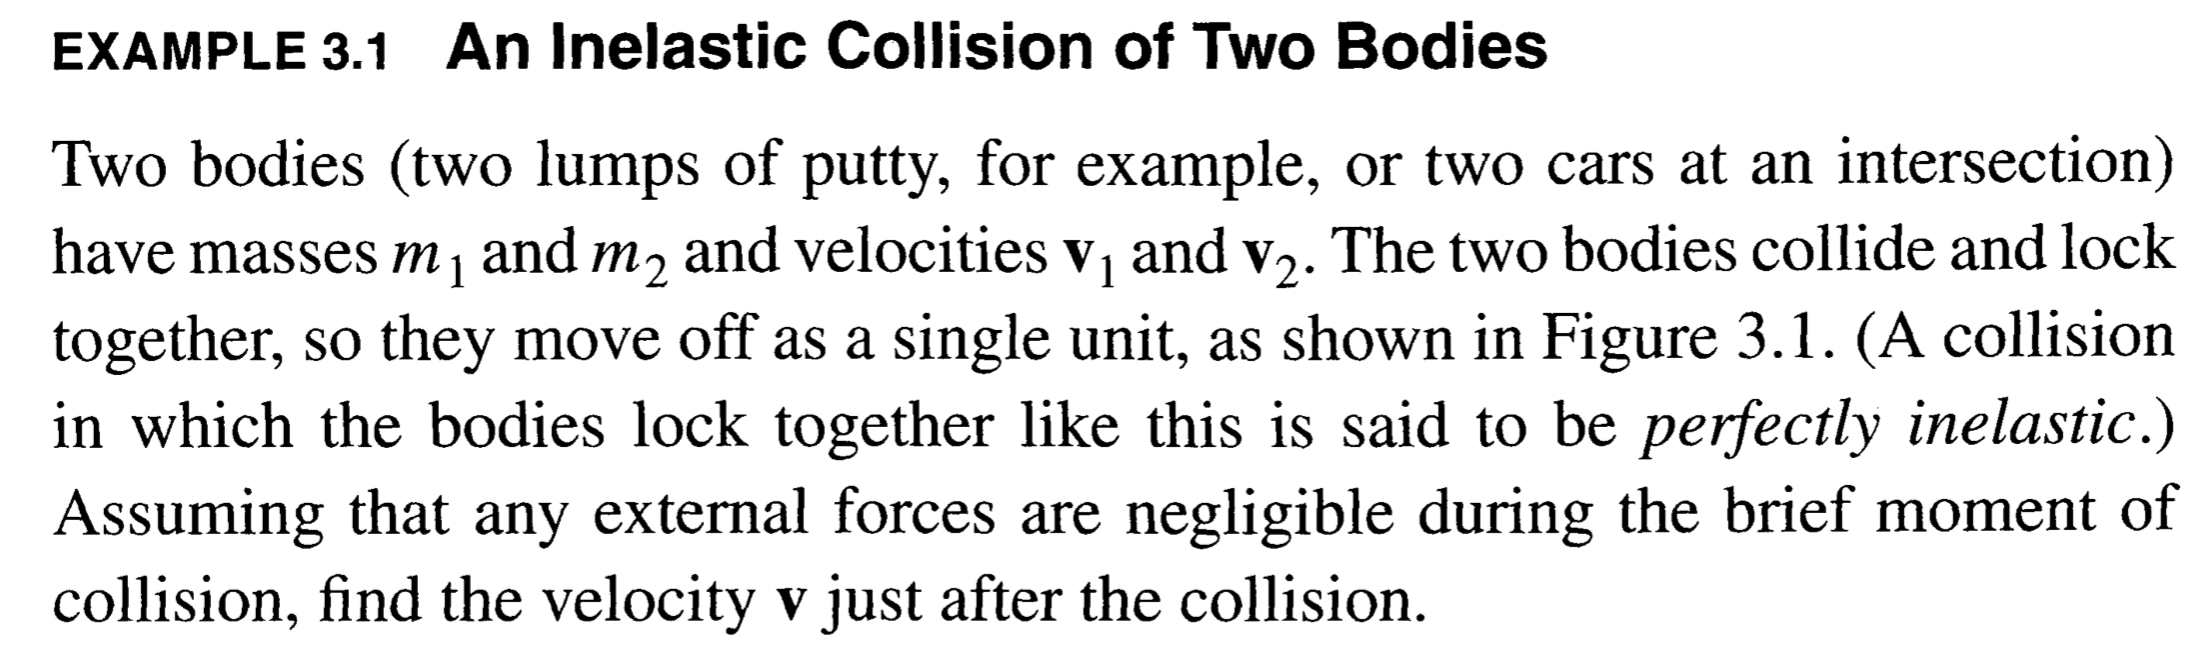
\includegraphics[width=400pt]{img/physics--classical-mechanics--taylor--sec-3-1.png}
\end{mdframed}

We have
\begin{align*}
  m_1\vec{v_1} + m_2\vec{v_2} &= (m_1 + m_2)\vec{v} \\
  \vec{v} &= \frac{m_1\vec{v_1} + m_2\vec{v_2}}{m_1 + m_2} \\
          &= \alpha\vec{v_1} + (1 - \alpha)\vec{v_2},
\end{align*}
where $\alpha = \frac{m_1}{m_1 + m_2}$.


\red{What happens if we do this with conservation of energy? Suppose we are in 1-D}
\begin{align*}
  \frac{1}{2}m_1v_1^2 + \frac{1}{2}m_2v_2^2 &= \frac{1}{2}(m_1 + m_2)v^2 \\
  v                                        &= \sqrt{\frac{m_1v_1^2 + m_2v_2^2}{m_1 + m_2}}.
\end{align*}
So, letting $v_M$ and $v_E$ be the momentum- and energy- based post-collision velocity answers, we
have
\begin{align*}
  v_E^2 &= \alpha v_1^2 + (1 - \alpha)v_2^2 \\
  v_M^2 &= \(\alpha v_1 + (1 - \alpha)v_2\)^2.
\end{align*}
Since $x \mapsto x^2$ is a convex function (\ref{convexity}), we have that $v_E > v_M$.

\red{Why is this -- why does assuming conservation of kinetic energy lead to a higher post-collision
  velocity than assuming conservation of momentum?}  \blue{Is this because squashing the lumps of
  putty together necessarily loses KE, so if we assume KE is conserved then we are overestimating
  the post-collision KE, which is why the post-collision velocity $v_E$ is greater than the estimate
  $v_M$ based on conservation of momentum?}




\subsubsection*{Example: Elastic collision (Morin p.162)}

\begin{mdframed}
  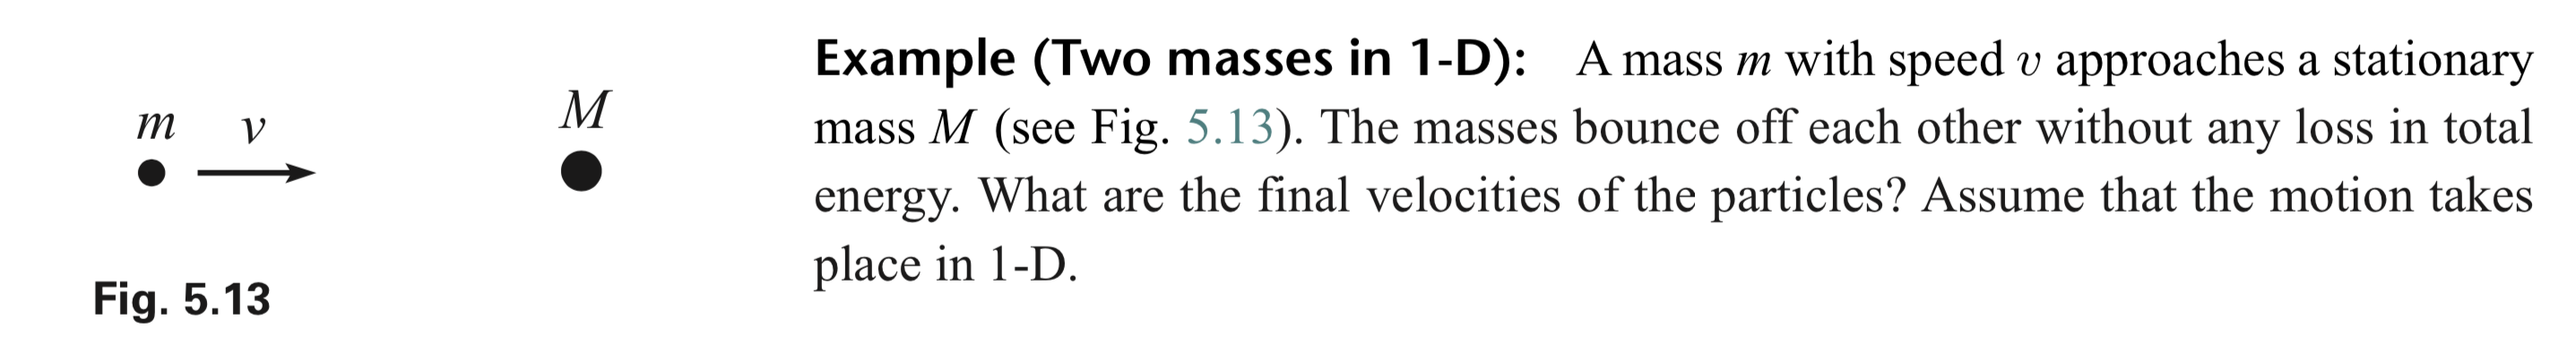
\includegraphics[width=400pt]{img/physics--classical-mechanics--morin--sec-5-6-ex.png}
\end{mdframed}

This can be solved in two ways:
\begin{enumerate}
\item Using the center of mass (CM) frame (Morin p.164)
\item Using conservation of kinetic energy (Morin p. 164, )
\end{enumerate}

\section{Projectile motion}

A projectile of mass $m$ is released with velocity $v_0$ at an angle $\theta$ to the ground. There
is no air resistance.

Note that vertical and horizontal motion are independent of each other. The equations of motion are:

\begin{itemize}
\item {\bf Vertical}\\
  $\ddot{y}(t) = -g$, with initial condition $\dot{y}(0) = v_0\sin\theta$.
\end{itemize}

\subsection{Using integration / FTC to solve the equation of motion}
Informally, since the acceleration is constant, the solution for the velocity function must be
$\dot{y}(t) = v_0\sin\theta - gt$, and therefore by integration the solution for vertical
position is $y(t) = y_0 + v_0\sin\theta t -\frac{1}{2}gt^2$.

More formally, we want to identify the set of functions $y$ that are consistent with the facts:
\begin{align*}
  \ddot{y}(t) &= -g \\
  \dot{y}(0)  &= v_0 \\
  y(0)        &= y_0.
\end{align*}

The first step is to identify the set of first-derivative functions $\dot{y}$ that fit the
facts. Using only the fact that the second derivative is a constant $-g$, we conclude that the
first derivative can be any linear function: $\dot{y}(t) = C - gt$. Then using the initial
velocity, we narrow this further to $\dot{y}(t) = v_0 - gt$.

More formally... the ``antiderivative'' operation maps a single function to a (infinite) set of
functions.
\begin{align*}
  \int \ddot{y}(t) \dt = \int -g \dt = C - gt.
\end{align*}

But the operation of integration maps an $\R \to \R$ function to $\R$.

We have an $\R \to \R$ function $\ddot{y}(t) = -g$. Antidifferentiating tells us that a family of
linear velocity functions are consistent with the acceleration function. What does integration
tell us? It tells us the ``net amount'' of acceleration that has accumulated between time $0$ and
time $t$. (And the FTC tells us that antidifferentiating gives us a trick to find this net amount
easily.)

It's easier to think about velocity and distance. ``Net amount of accumulated velocity'',
i.e. area under the velocity graph, corresponds to net displacement. E.g. $70$ mph $\times$ $2$
hrs equals $140$ miles displacement. What does that familiar calculation correspond to formally?
$140$ miles displacement is saying $x(2) - x(0) = 140$. So the statement is that
\begin{align}
    x(t) - x(0) &= \int_{t'=0}^{t'=t} \dxdt(t') \dt' \label{pcm-ftc} \\
                &= \int_{t'=0}^{t'=t} 70 \dt'.       \nonumber
\end{align}
In this case, \eqref{pcm-ftc} is common sense, because the velocity is constant. But for an
arbitrary velocity function, it would be invoking the FTC.

To compute that integral we can either
\begin{enumerate}
\item Use common sense again: visualize it as the area of a rectangle with height $70$ and width
  $t$.
\item Invoke the FTC a second time: notice that area is increasing linearly with $t$ with a slope
  of $70$, so the answer to the integral is given by the difference in value at $0$ and at $t$ of
  some function which has a slope equal to the integrand. Obvious for a constant integrand, but
  the FTC says that that line of thought still holds when the integrand is any well-behaved
  function. In other words, we need to antidifferentiate: find a function that has derivative
  $70$. In other words, we need to solve a differential equation: $f' = 70$.
\end{enumerate}

So in the velocity/distance problem, the facts were
\begin{align*}
    \dot{x} &= 70 \\
    x(0)    &= 0,
\end{align*}
we wanted to know the function $x$, and we found the solution $x(t) = 70t$ by solving the equation
\begin{align*}
    x(t) - x(0) = \int_0^t 70 \dt.
\end{align*}

Returning to the vertical acceleration of the projectile, the area under the acceleration graph
corresponds to net change in velocity. Recall that the facts are
\begin{align*}
    \ddot{y}(t) &= -g \\
    \dot{y}(0)  &= v_0 \\
    y(0)        &= y_0.
  \end{align*}
  We want to know the function $y$. So, invoking the FTC, we write down the equation
  \begin{align*}
    \int_{t'=0}^{t'=t}\ddot{y}(t') \dt' &= \dot{y}(t) - \dot{y}(0) \\
    \int_{t'=0}^{t'=t}-g \dt' &= \dot{y}(t) - v_0.
\end{align*}
Then, to solve this equation, we invoke FTC again, identifying $-gt$ as an antiderivative, and
conclude that
\begin{align*}
    -gt'\Big|_{t'=0}^{t'=t} &= \dot{y}(t) - v_0 \\
    \dot{y}(t)                   &= v_0 - gt.
\end{align*}
Then, we repeat the procedure, writing down
\begin{align*}
    \int_{t'=0}^{t'=t}\dot{y}(t') \dt' &= y(t) - y(0) \\
    \int_{t'=0}^{t'=t}v_0 - gt \dt'    &= y(t) - y_0 \\
    v_0t' - \frac{1}{2}gt'^2\Big|_{t'=0}^{t'=t} &= y(t) - y_0 \\
    y(t) &= y_0 + v_0t - \frac{1}{2}gt^2.
\end{align*}

